\documentclass[11pt,a4paper]{article}
\usepackage[T1]{fontenc}\usepackage[utf8]{inputenc}\usepackage[brazil]{babel}
\usepackage{lmodern,microtype,amsmath,booktabs,array,graphicx,float,caption,xcolor,enumitem,fancyhdr,hyperref}
\usepackage[margin=1.9cm,top=1.9cm,bottom=1.9cm]{geometry}
\definecolor{navy}{HTML}{164E63}\definecolor{light}{HTML}{EDF4F6}
\hypersetup{colorlinks=true,linkcolor=navy,urlcolor=navy,pdftitle={Quando fazer carrego? Doze testes e extensões},pdfauthor={Macroeconomia Aplicada}}
\setlength{\parindent}{0pt}\setlength{\parskip}{5pt}\setlength{\emergencystretch}{3em}
\setlength{\tabcolsep}{5pt}\renewcommand{\arraystretch}{1.12}
\setlength{\intextsep}{6pt}\setlength{\textfloatsep}{8pt}
\captionsetup{font=small,labelfont={bf,color=navy},skip=4pt}
\setlist{nosep}\pagestyle{fancy}\fancyhf{}\setlength{\headheight}{14pt}
\fancyhead[L]{\small\color{navy}Quando fazer carrego?}\fancyhead[R]{\small Estudo secundário | 2026}
\fancyfoot[C]{\small\thepage}
\begin{document}

\thispagestyle{empty}
{\large\color{navy}MACROECONOMIA APLICADA \quad | \quad ESTUDO SECUNDÁRIO}
\vspace{1cm}

{\Huge\bfseries\color{navy}Quando fazer carrego?}
\vspace{.35cm}

{\Large Doze testes sobre previsão cambial, risco e portfólio}
\vspace{.5cm}

Real, euro, iene, libra, dólar canadense e coroa sueca.\\
Resultados até agosto de 2026. Relatório preparado em 10 de setembro de 2026.
\vspace{.6cm}

\textbf{Resultado central.} A previsão tem algum potencial para regular a exposição ao carry e o hedge de ativos em dólar. Nesta amostra, ela não demonstrou capacidade adicional de antecipar perdas do carry, inflação ou retornos locais de ações. Uma previsão de valorização favorável não equivale a comprovar que o carrego ficou seguro.

\textbf{O que merece aprofundamento.} Em datas comuns, de janeiro de 2013 a agosto de 2026, dimensionar gradualmente o carry elevou o Sharpe de 0,661 para 0,728. Uma variação com retorno previsto mínimo de 2\% ao ano e média de seis meses alcançou Sharpe 0,883, com exposição em 35,4\% dos meses. Esses ganhos foram encontrados explorando a mesma história; não são validação independente.

\textbf{Hedge sem abandonar a bolsa.} Manter SPY e ajustar só sua proteção cambial preservou o retorno do ativo americano. Um hedge gradual teve CAGR em reais de 25,23\%, contra 23,45\% do hedge fixo de 50\%, mas o intervalo para a diferença de retorno médio inclui zero. O hedge fixo já explica boa parte da proteção.

\textbf{O que foi entregue.} Doze famílias de testes; 32 carteiras e controles na rodada principal; 43 especificações de carry e 62 combinações de ativo, hedge e custo na exploração; 18 alvos preditivos, cada um comparando controles, controles + EJR e controles + q. Resultados integrais em CSV, código, dados adicionais e auditoria acompanham este PDF.

\vfill
\colorbox{light}{\parbox{.94\linewidth}{\textbf{Documento separado.} O relatório principal, suas figuras, seus dados e seu pacote de entrega permanecem idênticos. Esta extensão é exploratória e não altera as conclusões originais.}}

\clearpage

\section*{Como os testes foram construídos}
O objeto é o valor da informação cambial em decisões de investimento, sem interpretação causal. A especificação principal reaproveita a previsão EJR de 60 meses, estimada em expansão. EJR refere-se a Eichenbaum, Johannsen e Rebelo; a versão da aula e as diferenças da replicação estão documentadas no relatório principal.

Se $S$ é a quantidade de moeda local por dólar, usamos $q=\log S+\log P_{US}-\log P_{local}$. A previsão $f_{t,60}$ é a variação esperada de $\log S$ em 60 meses. O componente cambial mensal para uma aplicação estrangeira avaliada em USD é $-f_{t,60}/60$. O escore de retorno esperado é
\[ a_{c,t}=\underbrace{\log(1+i^m_{c,t})-\log(1+i^m_{US,t})}_{k_{c,t}:\ \text{diferencial de juros}}-f_{c,t,60}/60. \]
Dividir a previsão longa por 60 é uma regra de alocação, não uma prova de previsibilidade mensal. Os juros anuais são convertidos geometricamente para o mês. A carteira carry compra as duas moedas de maior diferencial e vende as duas de menor diferencial, com pesos +25\%, +25\%, -25\%, -25\%.

\textbf{Contabilidade.} Todas as carteiras cambiais recebem caixa USD, resultado cambial, diferencial de juros e pagam custos. O retorno de um ativo estrangeiro em USD é $(1+i^m_c)S_{t-1}/S_t-1$; a posição tem funding em USD. O fator de interação entre câmbio e juros é mantido. Não há uma estratégia que receba somente a variação do spot.

\textbf{Relógio da informação.} Sinal no fechamento $t$, execução no fechamento $t+1$, primeiro retorno contabilizado em $t+2$. CPI tem dois meses de defasagem e preenchimento de, no máximo, uma referência ausente com o passado. No EJR, o último retorno utilizado na estimação termina até $t-1$. Novos modelos só aprendem alvos completamente realizados, também com margem de um mês; inflação recebe mais dois meses de divulgação. Normalizações, medianas e percentis são calculados com o passado.

\textbf{Custos e implementação.} Custos de câmbio de uma via: BRL 10 bps; SEK 3 bps; EUR, JPY, GBP e CAD 2 bps. Adicional de empréstimo nas posições vendidas: 50 bps anuais. Há ajuste pelo desvio dos pesos e liquidação final. No hedge, custo base de rolagem de 2 bps por mês de notional protegido, testado também a 5 e 10 bps. ETFs têm 12 bps na entrada e saída.

\textbf{Amostras e limitações.} Carteiras principais: março de 2010 a agosto de 2026, 198 meses. Variações: janeiro de 2013 a agosto de 2026, 164 meses, para evitar diferenças de aquecimento; subdivisões 2013--2018 e 2019--2026. Nenhuma é uma amostra histórica ainda não vista. Taxas oficiais são aproximações de aplicações/funding; forwards são sintéticos, sem base cambial observada. Não estão incluídos impostos, restrições de margem, limites de capital e taxas individuais de execução. As séries são snapshots atuais, não arquivos completos de vintages em tempo real.

\clearpage

\section*{O que cada uma das 12 ideias mostrou}
\begin{enumerate}[leftmargin=1.7em,itemsep=8pt]
\item \textbf{Quando fazer carrego.} Exigir retorno total previsto positivo melhorou modestamente o resultado, ao evitar só sete meses. Exigir valorização cambial favorável ficou em caixa a maior parte do tempo.
\item \textbf{Quais posições manter.} Filtrar pares pelo retorno total preservou neutralidade, mas teve CAGR menor que carry puro. A diferença frente a exposição equivalente não é conclusiva.
\item \textbf{Quanto carregar.} Exposição gradual mostrou melhora moderada de retorno por risco, inclusive na janela comum; é uma candidata mais interessante que a troca do ranking de moedas.
\item \textbf{O câmbio vai consumir os juros?} Adicionar EJR piorou ligeiramente o Brier. Não há evidência de que o sinal reconheça melhor esse evento.
\item \textbf{O carry vai sofrer perda extrema?} Não melhorou as previsões de perdas mensais ou trimestrais. Eventos raros limitam bastante a inferência.
\item \textbf{O que acontece antes do vencimento?} Não melhorou previsões da perda máxima no caminho nem do tempo abaixo do preço de entrada. Horizontes longos deixam pouquíssimos episódios independentes.
\item \textbf{Concordância entre horizontes.} Os sinais por moeda concordaram em 100\% das observações comuns de 1, 3, 5 e 8 anos. Não são quatro confirmações independentes.
\item \textbf{Quando sair.} Saídas por desaparecimento do retorno previsto tiveram ganho pequeno frente à mesma estrutura de coortes. Não impediram o pior drawdown.
\item \textbf{Extremos e assimetria.} Filtrar apenas a ponta comprada funcionou melhor que exigir moeda cara na ponta vendida. Exigir simultaneamente os dois extremos não gerou operações nesta amostra.
\item \textbf{Hedge do ativo em dólar.} É uma aplicação economicamente distinta e útil: preserva SPY/BIL. Há candidatos interessantes, mas a vantagem do sinal sobre hedge fixo não ficou estatisticamente estabelecida.
\item \textbf{Prever inflação.} O sinal não reduziu o erro da inflação relativa em nenhum dos três horizontes testados.
\item \textbf{Prever outros ativos.} Ações não mostraram melhora. IMAB11 teve redução ínfima do erro anual, baseada em apenas 14 origens sobrepostas; insuficiente para uma conclusão.
\end{enumerate}

\clearpage
\section*{1--3. Entrada, seleção e tamanho do carry}\small\begin{center}\begin{tabular}{lrrrrr}\toprule
Regra & CAGR (\%) & Vol. (\%) & Sharpe & DD (\%) & Exp. (\%) \\ \midrule
Carry puro & 4,11 & 4,43 & 0,601 & -9,09 & 100,00 \\
Ranking por EJR + juros & 2,73 & 4,16 & 0,309 & -7,01 & 100,00 \\
Entrada por câmbio & 2,09 & 1,59 & 0,383 & -2,96 & 14,14 \\
Entrada por retorno total & 4,29 & 4,38 & 0,647 & -9,09 & 96,46 \\
Filtro por par: total & 3,69 & 3,97 & 0,566 & -7,93 & 74,49 \\
Filtro por par: câmbio & 2,55 & 2,08 & 0,508 & -8,31 & 24,49 \\
Exposição gradual & 4,18 & 3,92 & 0,693 & -8,83 & 83,65 \\
Exposição por volatilidade & 3,59 & 4,01 & 0,535 & -8,13 & 88,10 \\
Gradual + volatilidade & 3,69 & 3,54 & 0,632 & -8,10 & 73,85 \\
\bottomrule\end{tabular}\end{center}\normalsize

CAGR e volatilidade anuais; drawdown (DD) desde o pico do patrimônio em USD; exposição bruta média. O Sharpe usa excesso sobre caixa USD. O filtro agregado aplica a previsão à carteira carry original: $A_t=\sum_c w^{carry}_{c,t}a_{c,t}$. Entrada por câmbio usa somente $\sum w(-f/60)>0$ para decidir a exposição, mas recebe juros no retorno realizado. Entrada total usa $A_t>0$.

O filtro por pares compara a moeda de maior juro com a de menor juro, depois a segunda com a segunda menor; cada par aprovado mantém suas pernas de 25\%. Não há concentração automática dos pesos restantes. Exposição gradual usa $\min(1,\max(0,A_t/\operatorname{mediana}_{u<t}A_u))$, após 24 observações. A regra de volatilidade limita a exposição para uma meta de 4\% anual, sem alavancar acima de 1.
\begin{figure}[H]\centering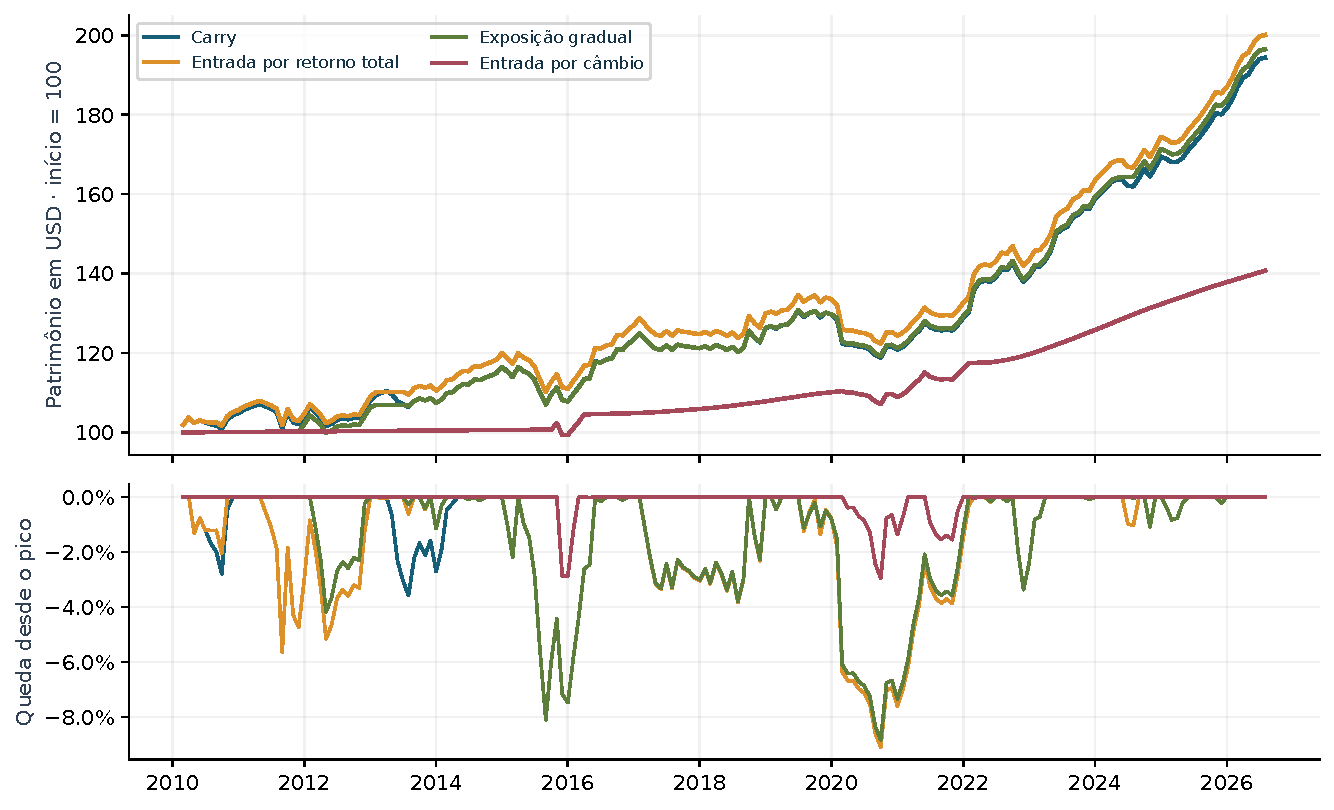
\includegraphics[width=.98\linewidth]{figures/carry_paths.pdf}\caption{Patrimônio com custos e quedas desde o pico. A exposição gradual passa inicialmente por aquecimento; a comparação em datas comuns aparece a seguir.}\end{figure}

\textbf{Leitura.} A entrada por câmbio reduz muito o drawdown porque praticamente não carrega: exposição de 14,1\%. Isso, isoladamente, não demonstra habilidade para antecipar perdas.

\clearpage
\section*{1. O sinal reconhece um carrego mais seguro?}\footnotesize\begin{center}\begin{tabular}{lrrrr}\toprule
Condição conhecida antes & Meses & Excesso a.a. (\%) & Meses negativos (\%) & Perda >2\% (\%) \\ \midrule
FX favorável & 28 & 4,28 & 42,86 & 3,57 \\
FX desfavorável & 170 & 2,37 & 38,82 & 2,94 \\
Total positivo & 191 & 2,92 & 38,22 & 3,14 \\
Total não positivo & 7 & -5,21 & 71,43 & 0,00 \\
Vol alta & 77 & 4,44 & 35,06 & 2,60 \\
Vol baixa & 121 & 1,49 & 42,15 & 3,31 \\
\bottomrule\end{tabular}\end{center}\normalsize

As linhas descrevem o carry puro nos meses classificados por informação disponível antes da execução. ``Excesso'' é média aritmética anualizada sobre caixa, não CAGR de uma sequência interrompida. Volatilidade alta/baixa é definida pela volatilidade móvel de 12 meses em relação à mediana passada.

Nos 28 meses com previsão cambial favorável, o retorno médio do carry foi maior, mas a frequência de meses negativos foi \textbf{42,9\%, contra 38,8\%} nos demais meses. A frequência de perdas superiores a 2\% também não caiu. Esses números não sustentam a afirmação de que a previsão tornou o risco cambial pequeno.

O sinal de retorno total ficou negativo em apenas sete meses. Foram meses ruins para carry, em média, mas representam pouquíssimos episódios. Desde 2019 a regra ficou sempre ligada e teve exatamente o mesmo retorno do carry puro.
\subsection*{Controle para simplesmente carregar menos}
\footnotesize\begin{center}\begin{tabular}{lrrr}\toprule
Regra & Comparação & Diferença (p.p./ano) & IC 95\% \\ \midrule
Entrada por câmbio & Carry & -2,05 & [-3,92; -0,04] \\
Entrada por câmbio & Mesma exposição média & 0,22 & [-0,39; 0,92] \\
Entrada por retorno total & Carry & 0,17 & [-0,02; 0,48] \\
Entrada por retorno total & Mesma exposição média & 0,27 & [0,04; 0,60] \\
Exposição gradual & Carry & 0,05 & [-0,67; 0,76] \\
Exposição gradual & Mesma exposição média & 0,48 & [-0,25; 1,14] \\
\bottomrule\end{tabular}\end{center}\normalsize

Intervalos percentis de bootstrap conjunto em blocos circulares de 12 meses, 1.999 reamostragens. São condicionais às estratégias já estimadas e não corrigidos por seleção de regras. O benchmark de mesma exposição usa a média \emph{ex post}, por isso é um diagnóstico, não uma estratégia implantável. Também foi executado o controle com média de exposição conhecida até o mês anterior; todos os resultados constam em \texttt{primary\_intervals.csv}.

\textbf{Placebo temporal.} Deslocar circularmente a sequência de exposições mantém aproximadamente sua persistência, mas altera o alinhamento com os retornos. Frações de deslocamentos com retorno superior ao observado: 25,1\% para entrada por câmbio, 10,1\% para entrada total e 11,6\% para exposição gradual. Não são p-valores de um experimento aleatório; reforçam a cautela quanto ao timing.

\clearpage
\section*{Variações de entrada e tamanho: onde há potencial}\small\begin{center}\begin{tabular}{lrrrrr}\toprule
Regra & CAGR (\%) & Vol. (\%) & Sharpe & DD (\%) & Exp. (\%) \\ \midrule
Carry & 4,55 & 4,23 & 0,661 & -9,09 & 100,00 \\
Total > 0 & 4,71 & 4,18 & 0,705 & -9,09 & 96,95 \\
Total > 2\%, média 6m & 4,32 & 2,91 & 0,883 & -6,78 & 35,37 \\
Gradual, mediana passada & 4,76 & 4,12 & 0,728 & -8,83 & 93,75 \\
Gradual, referência 2\% & 4,53 & 3,76 & 0,738 & -8,10 & 78,53 \\
q bruto, coeficiente 0,5 & 4,41 & 3,62 & 0,733 & -8,09 & 79,26 \\
\bottomrule\end{tabular}\end{center}\normalsize
\begin{figure}[H]\centering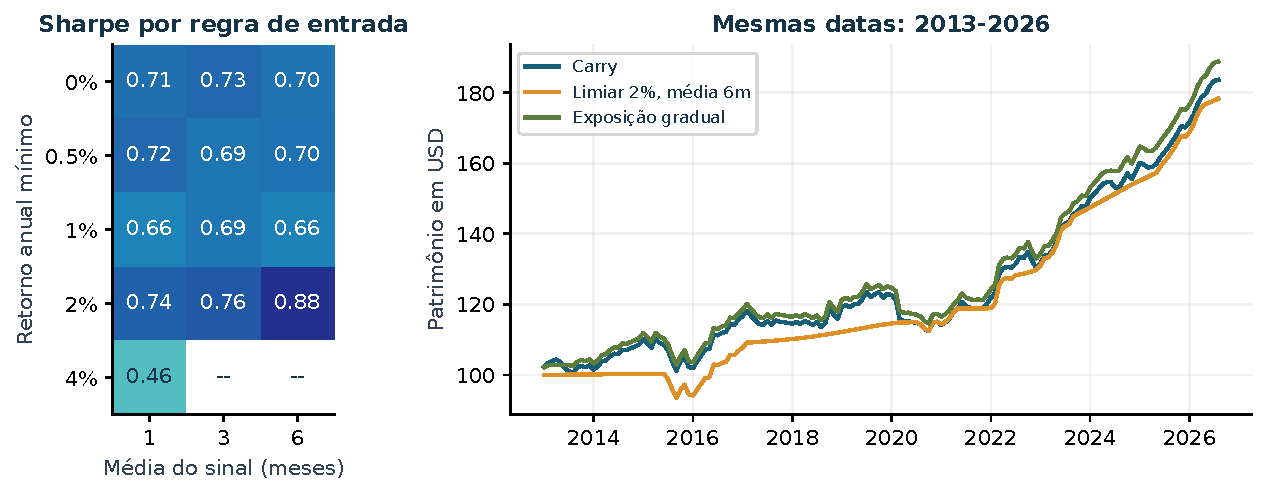
\includegraphics[width=.98\linewidth]{figures/timing_grid.pdf}\caption{Grade completa dos 15 filtros de entrada e patrimônio das regras centrais. Mesmas datas e custos. Célula sem Sharpe significa ausência de exposição.}\end{figure}

O melhor Sharpe da grade de entrada foi 0,883: limiar de 2\% e média de seis meses. A regra alcançou CAGR 4,32\%, abaixo dos 4,55\% do carry, mas com volatilidade de 2,91\% contra 4,23\%. Em 2013--2018, seu Sharpe foi 0,421, abaixo de 0,445 do carry; em 2019--2026, foi 1,385 contra 0,852. O ganho concentra-se no trecho recente. O IC de 95\% para a diferença de retorno médio anual frente ao carry é [-1,87; 1,39] p.p., em blocos de 12 meses. A regra também foi testada com custos duplicados, no apêndice.

A exposição gradual por mediana teve Sharpe 0,524 e 0,908 nas duas subdivisões, contra 0,445 e 0,852 do carry. Seu ganho é menor, porém aparece nos dois trechos. Uma regra simples com q bruto alcançou Sharpe 0,733: parte do resultado não depende da estimação EJR.

\textbf{Limite da descoberta.} Esses parâmetros foram examinados após a primeira rodada. Os apêndices incluem todos os resultados, inclusive regras que não operam e alavancagem de 1,5 vez, que ampliou perdas. Os intervalos de diferença de retorno médio frente ao carry, com blocos de 12 e 36 meses, estão em \texttt{variation\_intervals.csv}; não autorizam declarar a regra vencedora comprovada.

\clearpage
\section*{4--5. Antecipar perda de carrego e eventos extremos}\small\begin{center}\begin{tabular}{lrrrr}\toprule
Alvo / horizonte & Datas & EJR / base & q / base & p Holm \\ \midrule
Carrego consumido / 12m & 138 & 1,004 & 1,001 & 1,000 \\
Perda >2\% / 1m & 160 & 1,003 & 1,004 & 1,000 \\
Perda >4\% / 3m & 156 & 1,011 & 1,009 & 1,000 \\
\bottomrule\end{tabular}\end{center}\normalsize

Números abaixo de 1 indicariam melhora da raiz do Brier; acima de 1 indicam piora. ``q / base'' acrescenta o desvio real bruto aos mesmos controles. P-valores bilaterais HAC com ajuste Holm na família de comparações preditivas, incluindo as duas janelas de avaliação.

\textbf{Teste 4.} Para cada moeda, fixa-se o sentido do carry contra USD no instante do sinal. O evento ocorre quando a variação cambial adversa supera o diferencial de juros efetivamente acumulado nos 12 meses seguintes. É um diagnóstico logarítmico antes de custos; o lado do trade não muda durante o horizonte. A amostra avaliada tem 138 datas e 828 pares moeda-data, de fevereiro de 2014 a julho de 2025.

\textbf{Teste 5.} Os eventos são perdas do excesso líquido da carteira carry maiores que 2\% em um mês ou 4\% em três meses. O horizonte trimestral acumula geometricamente o excesso mensal. Custos e funding estão presentes. Os limites são fixos. Há apenas cinco eventos avaliados em cada horizonte: uma classificação que sempre dissesse ``não haverá perda extrema'' já acertaria cerca de 97\% das datas.
\begin{figure}[H]\centering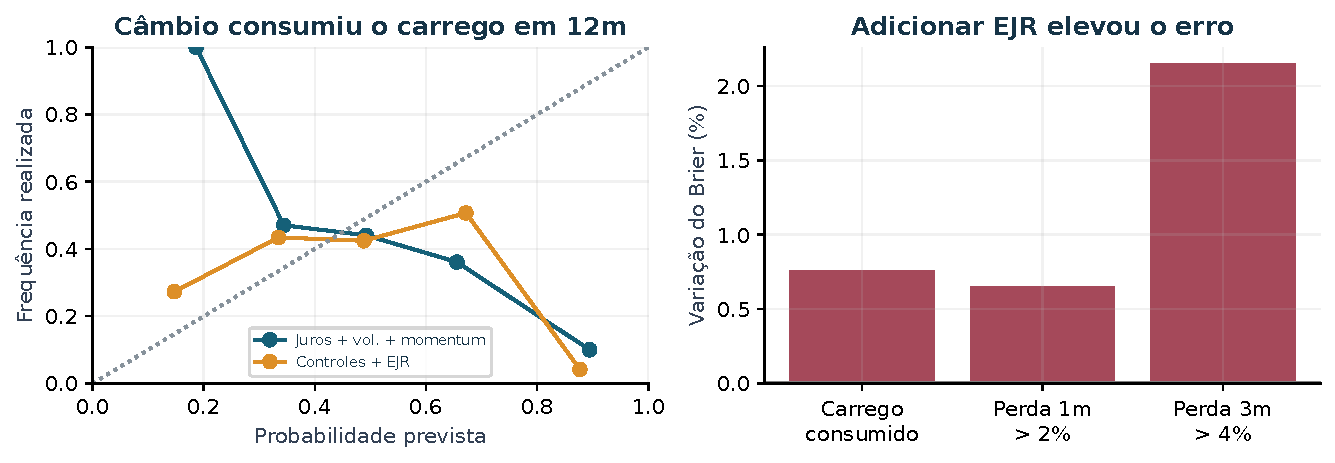
\includegraphics[width=.98\linewidth]{figures/risk_forecasts.pdf}\caption{Calibração em cinco faixas fixas de probabilidade (painel esquerdo). Erro relativo ao acrescentar EJR (direita); valores positivos são piora.}\end{figure}

\textbf{Modelos.} Probabilidade linear com ridge, limitada a [0,01; 0,99]. Controles: juros, volatilidade e momentum, orientados no sentido do carry; o painel tem interceptos por moeda. Penalização fixa 10, padronização somente no treino e mínimo de 36 datas/100 observações no painel. Não houve busca de hiperparâmetros. O modelo-base do teste 4 já apresenta discriminação fraca (AUC 0,484); EJR não a resgata (AUC 0,475).

\textbf{Conclusão.} Um sinal de retorno médio previsto não se transformou em um bom sinal de risco. A raridade e a concentração temporal das perdas extremas impedem tratar acurácia bruta elevada como evidência de sucesso.

\clearpage
\section*{6. Perdas no caminho e tempo de espera}\small\begin{center}\begin{tabular}{lrrrr}\toprule
Alvo / horizonte & Datas & EJR / base & q / base & p Holm \\ \midrule
Perda no caminho / 12m & 138 & 1,047 & 1,042 & 0,577 \\
Tempo submerso / 12m & 138 & 1,012 & 1,010 & 1,000 \\
Perda no caminho / 36m & 90 & 1,125 & 1,173 & -- \\
Tempo submerso / 36m & 90 & 1,091 & 1,129 & -- \\
Perda no caminho / 60m & 42 & 1,408 & 1,453 & -- \\
Tempo submerso / 60m & 42 & 1,402 & 1,463 & -- \\
\bottomrule\end{tabular}\end{center}\normalsize

Para cada moeda, o sentido inicial do carry contra USD é mantido por 12, 36 ou 60 meses. O primeiro alvo é a maior perda acumulada em log-retorno relativo ao caixa desde a entrada; o segundo é a proporção de meses em que esse acumulado ficou negativo. Incluem juros realizados e câmbio, antes de custos de execução e spread adicional de empréstimo.

Esse teste responde a uma questão diferente da rentabilidade no vencimento: \emph{mesmo que a moeda se ajuste em cinco anos, o investidor teria suportado a trajetória?} Não se assume que ele teria liquidez ou margem ilimitadas para atravessá-la.
\begin{figure}[H]\centering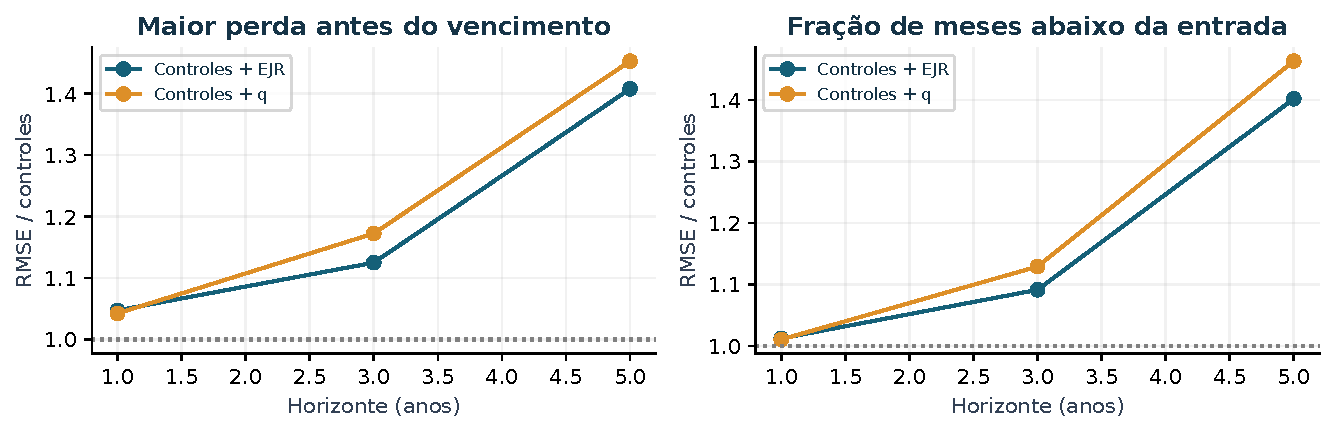
\includegraphics[width=.98\linewidth]{figures/path_prediction.pdf}\caption{Adicionar EJR não reduziu os erros de trajetória. Previsões de perda são limitadas a valores não negativos e de tempo submerso a [0,1].}\end{figure}

Os modelos são regressões ridge em expansão, com os mesmos controles do teste 4. Na previsão de perda em 60 meses, EJR elevou o RMSE em aproximadamente 40,8\%; na fração submersa, em 40,2\%. Esses resultados são desfavoráveis, mas não devem receber precisão estatística artificial.

\textbf{Poucos episódios independentes.} Há 42 origens mensais para os alvos de cinco anos e 90 para três anos, com forte sobreposição. Um painel de seis moedas não transforma 42 datas em 252 episódios independentes. Por isso não reportamos p-valor HAC quando existem menos de três blocos do horizonte ou menos de 36 datas. Os resultados longos são descritivos.

\clearpage
\section*{7--9. Horizontes, saída e assimetria}\small\begin{center}\begin{tabular}{lrrrrr}\toprule
Regra & CAGR (\%) & Vol. (\%) & Sharpe & DD (\%) & Exp. (\%) \\ \midrule
Carry & 4,11 & 4,43 & 0,601 & -9,09 & 100,00 \\
Concordância 4/4 & 2,51 & 1,72 & 0,421 & -2,96 & 17,07 \\
Concordância 3/4 & 2,51 & 1,72 & 0,421 & -2,96 & 17,07 \\
Coortes: prazo fixo & 3,55 & 4,27 & 0,495 & -9,92 & 97,20 \\
Coortes: sair se total < 0 & 3,66 & 4,10 & 0,539 & -9,92 & 89,08 \\
Coortes: reversão & 3,59 & 4,11 & 0,523 & -9,92 & 89,84 \\
Dois extremos & 1,50 & 0,52 & -- & 0,00 & 0,00 \\
Extremo na comprada & 3,51 & 3,65 & 0,565 & -9,09 & 61,11 \\
Extremo na vendida & 1,74 & 1,90 & 0,137 & -4,99 & 9,09 \\
\bottomrule\end{tabular}\end{center}\normalsize

\textbf{Teste 7: concordância.} As regras 4/4 e 3/4 operam só a partir da disponibilidade dos quatro horizontes; a tabela usa janeiro de 2013 em diante para elas. O carry nas mesmas datas tem CAGR 4,55\%, Sharpe 0,661 e DD -9,09\%. Não comparar seus CAGR diretamente com os 4,11\% da linha carry, que começa em 2010.

No painel comum de 166 sinais mensais, as direções previstas por moeda nos horizontes 12, 36, 60 e 96 meses concordam em 100\% dos casos. Os horizontes compartilham o mesmo desvio $q_t-\bar q_t$ e as inclinações estimadas mantêm o mesmo sinal. A concordância não constitui uma nova fonte de informação; ambos os filtros geraram o mesmo portfólio. O filtro de câmbio agregado também foi idêntico ao filtro que usa o q bruto.

\textbf{Teste 8: saída.} Uma nova coorte recebe 1/12 do orçamento por mês e mantém as moedas escolhidas na entrada por até 12 meses. O orçamento e os pesos dentro das coortes são mantidos como fração do NAV, portanto não se trata de comprar e esquecer a quantidade física. Comparações: vencimento fixo, sair quando o retorno esperado da coorte deixa de ser positivo e sair quando ele inverte o sinal inicial. Coortes encerradas ficam em caixa até o prazo original; não há reinvestimento oportunista dentro da mesma coorte.

Sair por retorno total elevou o CAGR de 3,55\% para 3,66\%, mas manteve o drawdown de -9,92\%. Desde 2019, as três regras tiveram retornos iguais. Não apareceu uma regra robusta de saída antecipada.

\textbf{Teste 9: extremos.} Percentis de cada moeda são calculados usando apenas sua história disponível. Exige-se q acima do percentil 70 para a ponta comprada, abaixo do percentil 30 para a vendida, ou ambos; o par mantém financiamento coerente. Exigir ambos não aprovou nenhum par: o resultado é caixa USD, não sucesso de proteção. A ponta comprada produziu maior atividade e retorno; filtrar a vendida quase eliminou a exposição. A assimetria observada não prova um efeito estrutural, pois os países e seus regimes de juros diferem.

\clearpage
\section*{10. Proteger o câmbio mantendo o ativo em dólar}
Aqui a carteira mantém 100\% de BIL ou SPY e escolhe a fração $H$ do notional inicial em USD que será vendida a termo por um mês. Não vende SPY para trocar por caixa. Os resultados são em reais, com dividendos reinvestidos nos preços ajustados.
\[ r^{BRL}_{t}=(1+r^{USD}_{A,t})\frac{S_t}{S_{t-1}}-1+H_{t-2}\left(\frac{F_{t-1,t}}{S_{t-1}}-\frac{S_t}{S_{t-1}}\right)-\text{custos}. \]
O forward sintético usa $F/S=(1+i^m_{BR})/(1+i^m_{US})$. O diferencial de juros entra no preço do hedge: não é proteção gratuita. ``Sinal cambial'' protege se $f_{BR,60}<0$; ``sinal com juros'' protege se $f_{BR,60}/60<k_{BR}$. Este último compara a valorização prevista do dólar com seu prêmio a termo.
\small\begin{center}\begin{tabular}{lrrrr}\toprule
Ativo / hedge & CAGR (\%) & Vol. (\%) & DD (\%) & Hedge médio (\%) \\ \midrule
BIL / nenhum & 7,95 & 15,03 & -23,53 & 0,00 \\
BIL / 50\% & 9,07 & 7,51 & -7,99 & 50,00 \\
BIL / 100\% & 9,60 & 0,96 & 0,00 & 100,00 \\
BIL / sinal cambial & 9,63 & 9,45 & -14,26 & 57,58 \\
BIL / sinal com juros & 9,10 & 5,78 & -14,26 & 86,87 \\
SPY / nenhum & 21,91 & 16,45 & -26,34 & 0,00 \\
SPY / 50\% & 22,67 & 13,54 & -22,61 & 50,00 \\
SPY / 100\% & 22,75 & 14,50 & -21,24 & 100,00 \\
SPY / sinal cambial & 23,15 & 15,41 & -21,24 & 57,58 \\
SPY / sinal com juros & 22,43 & 14,23 & -21,24 & 86,87 \\
\bottomrule\end{tabular}\end{center}\normalsize

Amostra de março de 2010 a agosto de 2026. DD é em reais. A proteção recai sobre o notional do ativo na abertura do mês, e não sobre seu valor final desconhecido; por isso resta a interação entre retorno do ativo e câmbio. Forwards efetivamente negociados, base cambial e margens não foram observados.

\textbf{Interpretação.} O hedge de SPY preserva a exposição à bolsa americana. A escolha entre fundos americanos e caixa brasileiro do relatório original misturava alocação de ativos e exposição cambial; esta extensão isola melhor a segunda decisão. Mesmo assim, um hedge fixo pode ser bastante competitivo: 50\% teve Sharpe 0,871 no período integral, acima de 0,812 do sinal cambial binário.

Para BIL totalmente protegido, o Sharpe contra caixa brasileiro fica muito negativo porque o excesso médio é ligeiramente negativo e sua volatilidade é minúscula. Não significa uma perda de patrimônio de magnitude comparável: o CAGR foi positivo e o drawdown mensal observado foi zero. Nesse caso, retorno excedente e custos são mais informativos que o Sharpe isolado.

\clearpage
\section*{10. Variações do hedge e risco do portfólio}\begin{figure}[H]\centering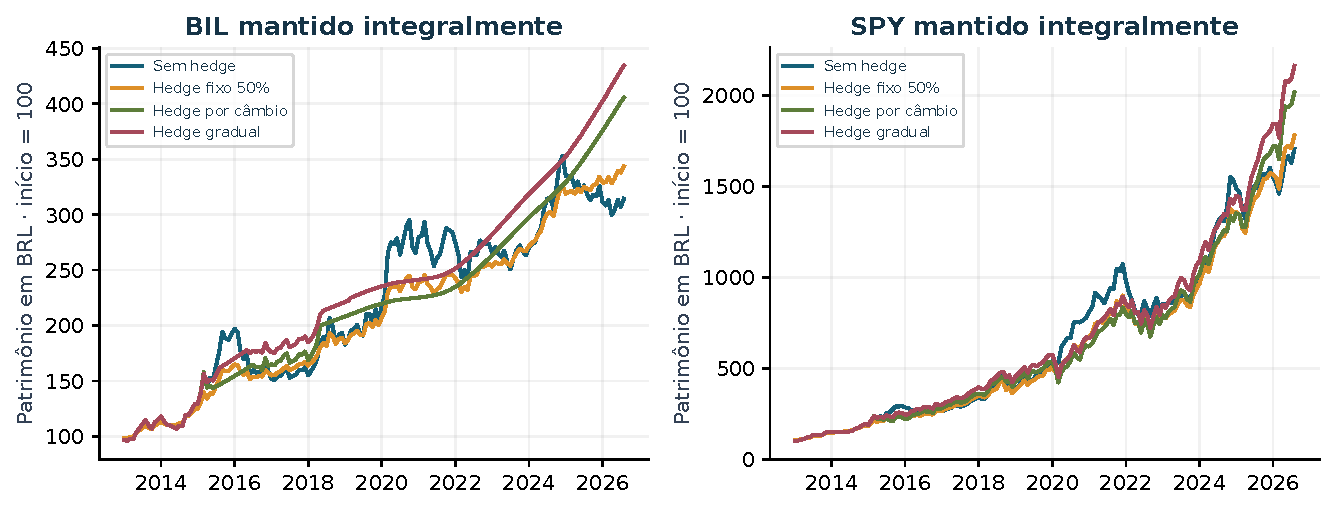
\includegraphics[width=.98\linewidth]{figures/hedge_paths.pdf}\caption{Comparação com exposição permanente ao mesmo ETF, janeiro de 2013 a agosto de 2026.}\end{figure}
\begin{figure}[H]\centering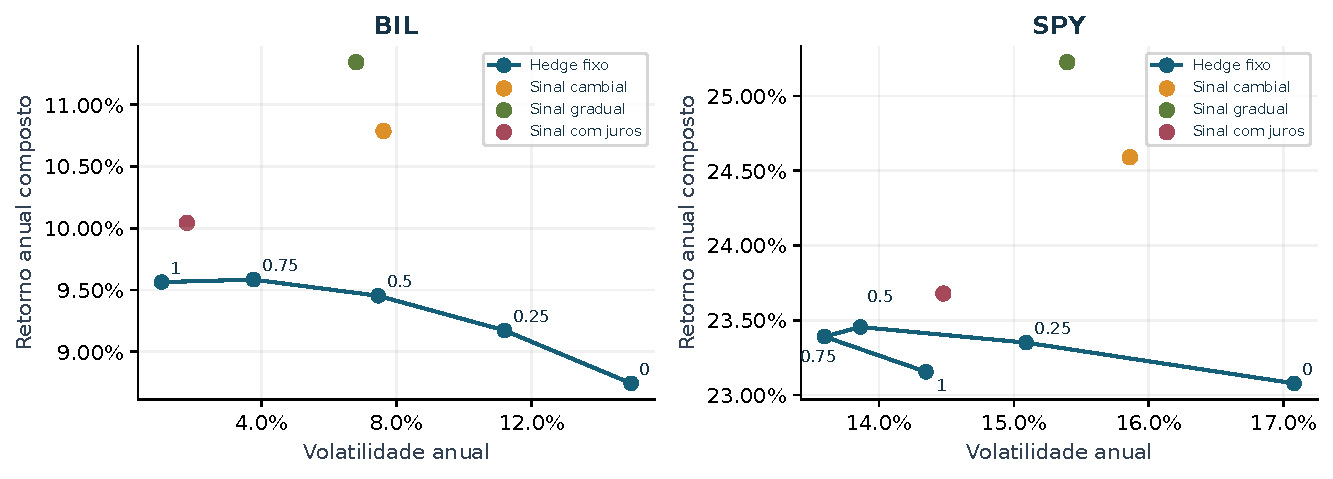
\includegraphics[width=.98\linewidth]{figures/hedge_frontier.pdf}\caption{Hedges fixos entre 0 e 1 versus regras condicionais. Cada ponto usa exatamente a mesma amostra; a curva conecta proporções fixas, não uma fronteira ótima estimada.}\end{figure}

O hedge gradual define $H_t=\operatorname{clip}(0,5-12f_{BR,60}/(60\times0,04),0,1)$: interpola entre proteção total para previsão anual de dólar menor que -2\% e nenhuma proteção acima de +2\%. Não foi calibrado para maximizar retorno.

Em SPY, a regra gradual teve CAGR 25,23\%, volatilidade 15,40\% e Sharpe 0,925, contra 23,45\%, 13,86\% e 0,901 para hedge fixo de 50\%. Em BIL, teve CAGR 11,34\%, contra 9,56\% com hedge total. Isso é potencial econômico, mas os intervalos ainda são largos. O sinal binário cambial ficou em proteção total desde 2019, sem acrescentar timing nesse trecho.

\clearpage
\section*{10. Quanto da vantagem do hedge é confiável?}\small\begin{center}\begin{tabular}{lrrr}\toprule
Ativo & Referência & Dif. média (p.p./ano) & IC 95\% \\ \midrule
BIL & Hedge 50\% & 1,68 & [-1,83; 4,79] \\
BIL & Hedge 100\% & 1,84 & [-1,43; 5,83] \\
BIL & Hedge médio ex post & 1,75 & [-0,96; 4,59] \\
SPY & Hedge 50\% & 1,68 & [-1,92; 5,00] \\
SPY & Hedge 100\% & 1,84 & [-1,67; 6,22] \\
SPY & Hedge médio ex post & 1,75 & [-1,04; 4,58] \\
\bottomrule\end{tabular}\end{center}\normalsize

Diferença de médias aritméticas anuais do hedge gradual em relação à referência, com bootstrap em blocos de 12 meses. Não são diferenças de CAGR. O hedge médio ex post iguala a proporção média de proteção do próprio sinal gradual para um diagnóstico de exposição; não é uma regra ex ante.

Todos esses intervalos incluem zero. O maior CAGR observado não é prova de habilidade cambial. Como o hedge protege o mesmo notional inicial, a diferença aritmética entre duas regras de hedge é igual para BIL e SPY em cada mês; diferenças nos intervalos publicados refletem apenas sorteios bootstrap distintos. CAGR e risco total diferem porque o retorno do ativo é diferente.
\subsection*{Sensibilidade a custo de rolagem}
\footnotesize\begin{center}\begin{tabular}{lrrr}\toprule
Ativo / regra & Custo (bps/mês) & CAGR (\%) & Sharpe \\ \midrule
BIL / 50\% & 2 & 9,45 & -0,032 \\
BIL / 50\% & 5 & 9,26 & -0,056 \\
BIL / 50\% & 10 & 8,93 & -0,096 \\
BIL / cambial & 2 & 10,79 & 0,130 \\
BIL / cambial & 5 & 10,51 & 0,097 \\
BIL / cambial & 10 & 10,06 & 0,042 \\
BIL / gradual & 2 & 11,34 & 0,212 \\
BIL / gradual & 5 & 11,06 & 0,174 \\
BIL / gradual & 10 & 10,59 & 0,110 \\
SPY / 50\% & 2 & 23,45 & 0,901 \\
SPY / 50\% & 5 & 23,24 & 0,888 \\
SPY / 50\% & 10 & 22,87 & 0,867 \\
SPY / cambial & 2 & 24,59 & 0,869 \\
SPY / cambial & 5 & 24,28 & 0,853 \\
SPY / cambial & 10 & 23,77 & 0,827 \\
SPY / gradual & 2 & 25,23 & 0,925 \\
SPY / gradual & 5 & 24,91 & 0,908 \\
SPY / gradual & 10 & 24,38 & 0,880 \\
\bottomrule\end{tabular}\end{center}\normalsize

O custo é cobrado a cada mês sobre a fração protegida; há ainda os custos de entrada/saída do ETF. A persistência dos resultados frente a essa grade não resolve o risco de base cambial ou restrições de margem, que exigiriam preços e regras contratuais próprios.

\clearpage
\section*{11. O desvio cambial ajuda a prever inflação?}\small\begin{center}\begin{tabular}{lrrrr}\toprule
Alvo / horizonte & Datas & EJR / base & q / base & p Holm \\ \midrule
Inflação · 1 ano & 134 & 1,117 & 1,119 & 1,000 \\
Inflação · 3 anos & 86 & 1,058 & 1,076 & -- \\
Inflação · 5 anos & 38 & 1,320 & 1,339 & -- \\
\bottomrule\end{tabular}\end{center}\normalsize

O alvo é a inflação acumulada local menos americana entre a abertura do investimento e 12, 36 ou 60 meses depois, expressa em log anualizado. O treino respeita dois meses extras de divulgação do CPI. Os controles são inflação relativa passada de 12 meses (defasada), diferencial de juros e momentum cambial. O painel possui interceptos por moeda.

EJR não melhorou o RMSE: pioras de 11,7\%, 5,8\% e 32,0\%, aproximadamente, nos três horizontes. A versão com q bruto também é mostrada para evitar atribuir à transformação estimada uma informação que já estava no nível do câmbio real.

Este resultado é compatível, em direção, com a distinção feita por Eichenbaum, Johannsen e Rebelo entre previsibilidade de câmbio nominal e de inflação. Não é uma nova confirmação causal do mecanismo do artigo: a amostra, os alvos, os controles e a avaliação são diferentes. A revisão do working paper está disponível no NBER [1].
\section*{12. O sinal ajuda com títulos ou ações locais?}
\small\begin{center}\begin{tabular}{lrrrr}\toprule
Alvo / horizonte & Datas & EJR / base & q / base & p Holm \\ \midrule
IMAB11 · 1 mês & 35 & 1,002 & 1,001 & -- \\
IMAB11 · 1 ano & 14 & 0,997 & 0,985 & -- \\
VALE - Itaú · 1 mês & 159 & 1,006 & 1,007 & 1,000 \\
VALE - Itaú · 1 ano & 138 & 1,116 & 1,136 & 1,000 \\
Suzano - BB · 1 mês & 159 & 1,008 & 1,009 & 1,000 \\
Suzano - BB · 1 ano & 138 & 1,025 & 1,026 & 1,000 \\
\bottomrule\end{tabular}\end{center}\normalsize

IMAB11 representa títulos públicos brasileiros indexados à inflação [2]. O alvo é seu retorno em BRL acima do caixa brasileiro. Nos pares de ações, o alvo é o retorno ajustado em BRL de VALE3 menos ITUB4, ou SUZB3 menos BBAS3. Para 12 meses somam-se os spreads mensais; não se apresenta isso como patrimônio composto de uma carteira alavancada.

Controles: juros, inflação relativa passada, momentum do BOVA11 e momentum do próprio alvo. O uso de moeda local retira a conversão mecânica USD/BRL. Os pares têm fortes diferenças de setor, commodity, crédito e governança; não identificam um prêmio causal de ``exportadora versus empresa doméstica''.

EJR não ajudou os pares de ações. O RMSE anual de IMAB11 caiu somente 0,32\%, com \textbf{14 datas de avaliação sobrepostas}. Seu histórico começa em maio de 2019 e o aprendizado exige história adicional. Esse ganho é demasiado pequeno e a amostra demasiado curta para classificá-lo como oportunidade.

\clearpage
\section*{Outros alvos: visão conjunta e limites de inferência}\begin{figure}[H]\centering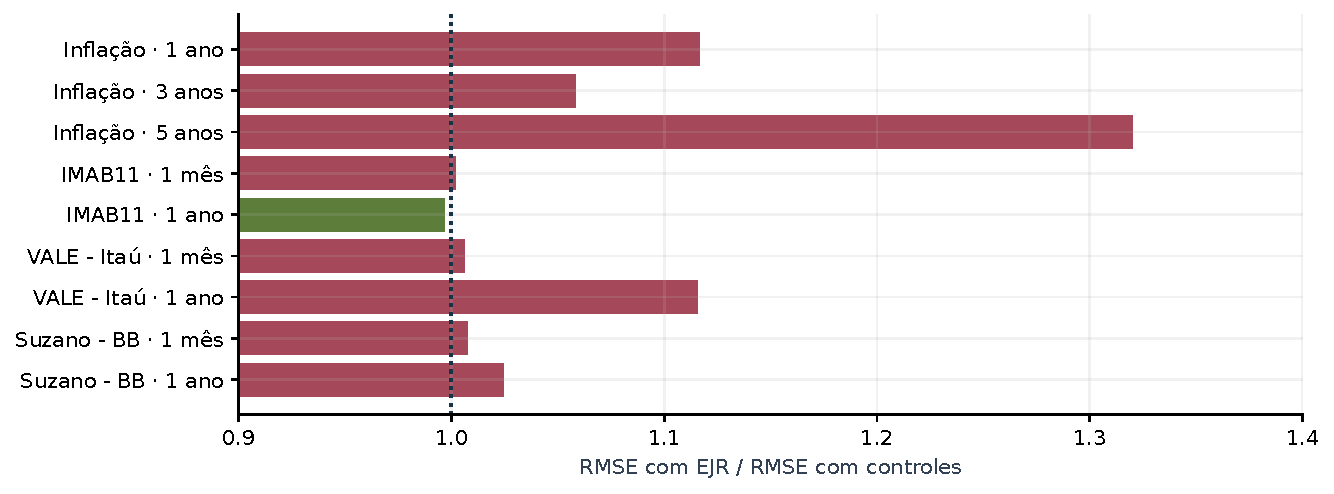
\includegraphics[width=.98\linewidth]{figures/other_targets.pdf}\caption{Erro com a previsão EJR relativo ao modelo com controles. A única barra abaixo de 1, IMAB11 em 12 meses, corresponde a 14 origens sobrepostas.}\end{figure}

\textbf{O que ``não melhorou'' significa aqui.} As conclusões se referem aos modelos, às variáveis, aos horizontes e às amostras explicitamente testados. Não provam impossibilidade de prever inflação, crises ou retornos de ativos. Os modelos de novos alvos foram mantidos simples e com regularização fixa; não procuramos algoritmos sucessivamente até encontrar um resultado favorável.

\textbf{Revisões e disponibilidade.} Há controle de divulgação por defasagem, mas não uma base integral de vintages. Preços ajustados de ações/ETFs são usados somente em retornos e momentum: não entram como nível macroeconômico. Mudanças históricas de metodologia, ajustes por eventos e revisões ainda podem afetar a replicação em tempo real. A escolha de empresas que hoje existem também torna o teste setorial um estudo de casos, não uma carteira representativa de todo o universo histórico.

\textbf{Inferência dependente do tempo.} Os erros de previsão são agregados por data antes de calcular HAC. Isso evita contar seis moedas expostas ao mesmo choque como seis experiências independentes. Os p-valores disponíveis são ajustados por Holm sobre todas as comparações EJR/q versus base, nos períodos integral e recente. A diferença de erro pode ser negativa: um p pequeno também pode indicar piora, não sucesso.

\textbf{Exploração de estratégias.} Os intervalos de retorno não corrigem a busca de parâmetros, não reestimam o modelo EJR dentro de cada reamostragem e são condicionais ao conjunto de sinais produzido. Os 1.999 blocos de 12 meses e a sensibilidade de 36 meses medem incerteza histórica parcial. Selecionar o melhor Sharpe entre dezenas de regras infla a impressão de desempenho; as grades completas são preservadas justamente para tornar essa seleção visível.

\textbf{Decisão para o trabalho.} Os resultados justificam discutir o uso da previsão como modulador de exposição e de hedge, acompanhado de benchmarks simples. Não justificam substituir a conclusão central por uma alegação de arbitragem ou de carry seguro. Uma próxima validação teria de congelar a regra e observar dados novos ou uma amostra externa verdadeiramente não usada na seleção.

\clearpage
\section*{Apêndice A1. Todas as variações de carry}Janeiro de 2013 a agosto de 2026. Nomes correspondem exatamente aos CSVs. CAGR, volatilidade, DD e exposição em porcentagem; Sharpe em unidade.\par \small\begin{center}\begin{tabular}{lrrrrr}\toprule
Regra & CAGR (\%) & Vol. (\%) & Sharpe & DD (\%) & Exp. (\%) \\ \midrule
Carry & 4,55 & 4,23 & 0,661 & -9,09 & 100,00 \\
Gate\_0\_ma1 & 4,71 & 4,18 & 0,705 & -9,09 & 96,95 \\
Gate\_0\_ma3 & 4,80 & 4,17 & 0,726 & -9,09 & 96,95 \\
Gate\_0\_ma6 & 4,67 & 4,17 & 0,697 & -9,09 & 97,56 \\
Gate\_0.005\_ma1 & 4,77 & 4,15 & 0,725 & -9,09 & 95,12 \\
Gate\_0.005\_ma3 & 4,65 & 4,17 & 0,694 & -9,09 & 95,73 \\
Gate\_0.005\_ma6 & 4,68 & 4,16 & 0,702 & -9,09 & 95,12 \\
Gate\_0.01\_ma1 & 4,41 & 4,05 & 0,659 & -8,15 & 85,37 \\
Gate\_0.01\_ma3 & 4,53 & 4,05 & 0,689 & -8,10 & 85,37 \\
Gate\_0.01\_ma6 & 4,47 & 4,11 & 0,660 & -8,10 & 89,02 \\
Gate\_0.02\_ma1 & 4,06 & 3,10 & 0,741 & -7,70 & 34,76 \\
Gate\_0.02\_ma3 & 3,99 & 2,93 & 0,763 & -8,14 & 34,76 \\
Gate\_0.02\_ma6 & 4,32 & 2,91 & 0,883 & -6,78 & 35,37 \\
Gate\_0.04\_ma1 & 2,14 & 0,87 & 0,462 & -0,03 & 1,83 \\
Gate\_0.04\_ma3 & 1,79 & 0,54 & -- & 0,00 & 0,00 \\
Gate\_0.04\_ma6 & 1,79 & 0,54 & -- & 0,00 & 0,00 \\
Size\_hist6\_cap0.5 & 3,29 & 2,14 & 0,718 & -4,22 & 48,28 \\
Size\_hist6\_cap1 & 4,76 & 4,12 & 0,728 & -8,83 & 93,75 \\
Size\_hist6\_cap1.5 & 6,02 & 5,71 & 0,747 & -12,03 & 122,89 \\
Size\_hist12\_cap0.5 & 3,29 & 2,14 & 0,718 & -4,22 & 48,28 \\
Size\_hist12\_cap1 & 4,76 & 4,12 & 0,728 & -8,83 & 93,75 \\
\bottomrule\end{tabular}\end{center}\normalsize

\texttt{Gate\_x\_maN}: limiar $100x$\% ao ano e média de $N$ meses. \texttt{Size\_histN\_capC}: mediana histórica com mínimo $N$ e exposição máxima $C$. \texttt{Size\_fixedx}: sinal dividido por $x$ anual, limitado a 1. \texttt{Rawq\_coefx}: troca o EJR por $xq/60$. Sufixo \texttt{2cost}: custos de câmbio duplicados; spread de empréstimo mantido. Linhas de alavancagem não são recomendações de operação.

O arquivo \texttt{variation\_metrics.csv} contém os subperíodos; os intervalos de 12/36 meses estão em \texttt{variation\_intervals.csv}. As regras de histórico mínimo 6/12/24 meses coincidem na janela comum porque todas já passaram pelo aquecimento; não são evidências independentes de robustez.

\clearpage
\section*{Apêndice A2. Todas as variações de carry}Janeiro de 2013 a agosto de 2026. Nomes correspondem exatamente aos CSVs. CAGR, volatilidade, DD e exposição em porcentagem; Sharpe em unidade.\par \small\begin{center}\begin{tabular}{lrrrrr}\toprule
Regra & CAGR (\%) & Vol. (\%) & Sharpe & DD (\%) & Exp. (\%) \\ \midrule
Size\_hist12\_cap1.5 & 6,02 & 5,71 & 0,747 & -12,03 & 122,89 \\
Size\_hist24\_cap0.5 & 3,29 & 2,14 & 0,718 & -4,22 & 48,28 \\
Size\_hist24\_cap1 & 4,76 & 4,12 & 0,728 & -8,83 & 93,75 \\
Size\_hist24\_cap1.5 & 6,02 & 5,71 & 0,747 & -12,03 & 122,89 \\
Size\_hist36\_cap0.5 & 3,29 & 2,14 & 0,718 & -4,22 & 48,28 \\
Size\_hist36\_cap1 & 4,76 & 4,12 & 0,728 & -8,83 & 93,75 \\
Size\_hist36\_cap1.5 & 6,01 & 5,71 & 0,746 & -12,03 & 122,89 \\
Size\_fixed0.01 & 4,66 & 4,13 & 0,702 & -9,16 & 94,35 \\
Size\_fixed0.02 & 4,53 & 3,76 & 0,738 & -8,10 & 78,53 \\
Size\_fixed0.04 & 3,58 & 2,41 & 0,759 & -5,16 & 44,70 \\
Rawq\_coef0 & 4,22 & 3,47 & 0,711 & -8,05 & 77,05 \\
Rawq\_coef0.25 & 4,31 & 3,53 & 0,724 & -8,07 & 78,27 \\
Rawq\_coef0.5 & 4,41 & 3,62 & 0,733 & -8,09 & 79,26 \\
Rawq\_coef1 & 4,38 & 3,76 & 0,698 & -8,10 & 77,44 \\
Rawq\_coef2 & 3,76 & 3,58 & 0,561 & -8,00 & 53,54 \\
Carry\_2cost & 4,52 & 4,23 & 0,654 & -9,12 & 100,00 \\
Gate\_0\_ma1\_2cost & 4,68 & 4,18 & 0,697 & -9,12 & 96,95 \\
Gate\_0.01\_ma3\_2cost & 4,49 & 4,05 & 0,678 & -8,12 & 85,37 \\
Gate\_0.02\_ma6\_2cost & 4,28 & 2,91 & 0,869 & -6,82 & 35,37 \\
Size\_hist24\_cap1\_2cost & 4,72 & 4,12 & 0,717 & -8,92 & 93,75 \\
Size\_fixed0.02\_2cost & 4,48 & 3,76 & 0,724 & -8,11 & 78,53 \\
Rawq\_coef0.5\_2cost & 4,37 & 3,62 & 0,723 & -8,09 & 79,26 \\
\bottomrule\end{tabular}\end{center}\normalsize

\texttt{Gate\_x\_maN}: limiar $100x$\% ao ano e média de $N$ meses. \texttt{Size\_histN\_capC}: mediana histórica com mínimo $N$ e exposição máxima $C$. \texttt{Size\_fixedx}: sinal dividido por $x$ anual, limitado a 1. \texttt{Rawq\_coefx}: troca o EJR por $xq/60$. Sufixo \texttt{2cost}: custos de câmbio duplicados; spread de empréstimo mantido. Linhas de alavancagem não são recomendações de operação.

O arquivo \texttt{variation\_metrics.csv} contém os subperíodos; os intervalos de 12/36 meses estão em \texttt{variation\_intervals.csv}. As regras de histórico mínimo 6/12/24 meses coincidem na janela comum porque todas já passaram pelo aquecimento; não são evidências independentes de robustez.

\clearpage
\section*{Apêndice B. Todas as variações de hedge: BIL}Janeiro de 2013 a agosto de 2026, retornos em reais.\par \footnotesize\begin{center}\begin{tabular}{lrrrrr}\toprule
Regra & bps/mês & CAGR (\%) & Vol. (\%) & Sharpe & DD (\%) \\ \midrule
Fixed\_0 & 2 & 8,74 & 14,95 & -0,005 & -23,53 \\
Fixed\_0 & 5 & 8,74 & 14,95 & -0,005 & -23,53 \\
Fixed\_0 & 10 & 8,74 & 14,95 & -0,005 & -23,53 \\
Fixed\_0.25 & 2 & 9,17 & 11,20 & -0,014 & -15,07 \\
Fixed\_0.5 & 2 & 9,45 & 7,46 & -0,032 & -7,99 \\
Fixed\_0.5 & 5 & 9,26 & 7,46 & -0,056 & -8,06 \\
Fixed\_0.5 & 10 & 8,93 & 7,46 & -0,096 & -8,18 \\
Fixed\_0.75 & 2 & 9,58 & 3,77 & -0,087 & -3,06 \\
Fixed\_1 & 2 & 9,56 & 1,04 & -3,918 & 0,00 \\
Fixed\_1 & 5 & 9,17 & 1,04 & -7,349 & 0,00 \\
Fixed\_1 & 10 & 8,53 & 1,04 & -13,069 & 0,00 \\
FX\_ma1\_b-0.01 & 2 & 11,69 & 8,24 & 0,225 & -9,58 \\
FX\_ma1\_b0 & 2 & 10,79 & 7,61 & 0,130 & -9,58 \\
FX\_ma1\_b0 & 5 & 10,51 & 7,62 & 0,097 & -9,58 \\
FX\_ma1\_b0 & 10 & 10,06 & 7,62 & 0,042 & -9,58 \\
FX\_ma1\_b0.01 & 2 & 12,07 & 6,23 & 0,333 & -9,58 \\
FX\_ma3\_b-0.01 & 2 & 11,82 & 8,43 & 0,237 & -9,58 \\
FX\_ma3\_b0 & 2 & 11,46 & 7,84 & 0,207 & -9,58 \\
FX\_ma3\_b0.01 & 2 & 10,92 & 7,32 & 0,148 & -9,58 \\
FX\_ma6\_b-0.01 & 2 & 13,69 & 9,24 & 0,406 & -9,58 \\
FX\_ma6\_b0 & 2 & 11,82 & 8,17 & 0,242 & -9,58 \\
FX\_ma6\_b0.01 & 2 & 11,38 & 7,12 & 0,211 & -9,58 \\
Total\_b-0.01 & 2 & 10,20 & 2,01 & 0,103 & -0,71 \\
Total\_b0 & 2 & 10,04 & 1,79 & 0,026 & -0,03 \\
Total\_b0.01 & 2 & 9,56 & 1,04 & -3,918 & 0,00 \\
Smooth\_FX & 2 & 11,34 & 6,80 & 0,212 & -9,58 \\
Smooth\_FX & 5 & 11,06 & 6,81 & 0,174 & -9,58 \\
Smooth\_FX & 10 & 10,59 & 6,82 & 0,110 & -9,58 \\
Matched\_expost & 2 & 9,57 & 4,57 & -0,067 & -3,86 \\
Matched\_smooth & 2 & 9,57 & 4,30 & -0,073 & -3,59 \\
Matched\_total & 2 & 9,57 & 1,04 & -1,283 & -0,03 \\
\bottomrule\end{tabular}\end{center}\normalsize

\texttt{Fixed\_x}: hedge fixo $x$. \texttt{FX\_maN\_bx}: média de $N$ meses e limiar anual $100x$\%. \texttt{Total\_bx}: compara a previsão com o diferencial de juros mais o limiar. \texttt{Smooth\_FX}: interpolação entre -2\% e +2\% anuais. \texttt{Matched\_expost/smooth/total}: hedge constante igual à proteção média observada do respectivo sinal binário/gradual/com juros, somente diagnóstico. Subperíodos em \texttt{hedge\_variations.csv}.

\clearpage
\section*{Apêndice B. Todas as variações de hedge: SPY}Janeiro de 2013 a agosto de 2026, retornos em reais.\par \footnotesize\begin{center}\begin{tabular}{lrrrrr}\toprule
Regra & bps/mês & CAGR (\%) & Vol. (\%) & Sharpe & DD (\%) \\ \midrule
Fixed\_0 & 2 & 23,08 & 17,08 & 0,740 & -26,34 \\
Fixed\_0 & 5 & 23,08 & 17,08 & 0,740 & -26,34 \\
Fixed\_0 & 10 & 23,08 & 17,08 & 0,740 & -26,34 \\
Fixed\_0.25 & 2 & 23,35 & 15,09 & 0,832 & -24,44 \\
Fixed\_0.5 & 2 & 23,45 & 13,86 & 0,901 & -22,61 \\
Fixed\_0.5 & 5 & 23,24 & 13,86 & 0,888 & -22,72 \\
Fixed\_0.5 & 10 & 22,87 & 13,86 & 0,867 & -22,89 \\
Fixed\_0.75 & 2 & 23,39 & 13,60 & 0,915 & -20,85 \\
Fixed\_1 & 2 & 23,15 & 14,35 & 0,865 & -21,24 \\
Fixed\_1 & 5 & 22,72 & 14,35 & 0,840 & -21,30 \\
Fixed\_1 & 10 & 22,00 & 14,35 & 0,798 & -21,38 \\
FX\_ma1\_b-0.01 & 2 & 25,63 & 15,97 & 0,917 & -21,24 \\
FX\_ma1\_b0 & 2 & 24,59 & 15,86 & 0,869 & -21,24 \\
FX\_ma1\_b0 & 5 & 24,28 & 15,86 & 0,853 & -21,30 \\
FX\_ma1\_b0 & 10 & 23,77 & 15,87 & 0,827 & -21,38 \\
FX\_ma1\_b0.01 & 2 & 26,02 & 15,22 & 0,976 & -21,24 \\
FX\_ma3\_b-0.01 & 2 & 25,78 & 16,04 & 0,922 & -21,24 \\
FX\_ma3\_b0 & 2 & 25,35 & 15,91 & 0,906 & -21,24 \\
FX\_ma3\_b0.01 & 2 & 24,75 & 15,63 & 0,888 & -21,24 \\
FX\_ma6\_b-0.01 & 2 & 27,88 & 16,43 & 1,007 & -21,24 \\
FX\_ma6\_b0 & 2 & 25,76 & 16,08 & 0,919 & -21,24 \\
FX\_ma6\_b0.01 & 2 & 25,28 & 15,47 & 0,925 & -21,24 \\
Total\_b-0.01 & 2 & 23,86 & 14,46 & 0,898 & -21,24 \\
Total\_b0 & 2 & 23,68 & 14,48 & 0,887 & -21,24 \\
Total\_b0.01 & 2 & 23,15 & 14,35 & 0,865 & -21,24 \\
Smooth\_FX & 2 & 25,23 & 15,40 & 0,925 & -21,24 \\
Smooth\_FX & 5 & 24,91 & 15,40 & 0,908 & -21,30 \\
Smooth\_FX & 10 & 24,38 & 15,41 & 0,880 & -21,38 \\
Matched\_expost & 2 & 23,42 & 13,56 & 0,918 & -21,23 \\
Matched\_smooth & 2 & 23,41 & 13,57 & 0,917 & -21,10 \\
Matched\_total & 2 & 23,18 & 14,26 & 0,870 & -20,90 \\
\bottomrule\end{tabular}\end{center}\normalsize

\texttt{Fixed\_x}: hedge fixo $x$. \texttt{FX\_maN\_bx}: média de $N$ meses e limiar anual $100x$\%. \texttt{Total\_bx}: compara a previsão com o diferencial de juros mais o limiar. \texttt{Smooth\_FX}: interpolação entre -2\% e +2\% anuais. \texttt{Matched\_expost/smooth/total}: hedge constante igual à proteção média observada do respectivo sinal binário/gradual/com juros, somente diagnóstico. Subperíodos em \texttt{hedge\_variations.csv}.

\clearpage

\section*{Auditoria, fontes e reprodução}
\textbf{22 verificações de integridade passaram.} Foram checados: reprodução do carry original; invariância das previsões históricas ao truncar a amostra ou corromper o futuro; defasagem de execução; neutralidade long--short; disponibilidade estritamente anterior de todos os rótulos usados no treino; mínimo de datas; efeito da defasagem do CPI; probabilidades válidas; sinais e identidade contábil do forward; preços positivos; calendário sem duplicações; hashes de seis novas fontes e preservação dos 99 arquivos originais.

\textbf{Limite da auditoria.} Os testes verificam a implementação e a cronologia declarada; não substituem dados históricos de vintages ou forwards negociados. Os coeficientes de EJR usam médias reais estimadas com a informação disponível em cada origem. As novas regressões padronizam variáveis apenas dentro do treino. Não foram usados limiares calculados a partir dos retornos futuros para criar os sinais.

\textbf{Arquivos.} Todo o código novo está em \texttt{secondary/}. \texttt{PROTOCOL.md} registra a primeira grade; \texttt{EXPLORATION.md}, as variações após resultados. \texttt{tables/} contém métricas, retornos, previsões individuais e a trilha de disponibilidade dos rótulos. \texttt{data/manifest.json} registra URLs e SHA-256 das séries adicionais. \texttt{original\_hashes.json} permite verificar a preservação do material principal. O PDF é compilado de \texttt{secondary/relatorio\_secundario.tex}.

\textbf{Reprodução local.} Executar, na raiz, com o Python do projeto: \texttt{secondary/analyze.py}, \texttt{secondary/variations.py}, \texttt{secondary/validate.py} e \texttt{secondary/build\_report.py}; depois compilar a fonte LaTeX com Tectonic. Não é necessário baixar novamente os dados. \texttt{secondary/run.ps1} automatiza a sequência. As dependências do Python são as do \texttt{requirements-lock.txt} original.

\subsection*{Fontes e escopo dos dados}
\begin{enumerate}[leftmargin=1.7em,itemsep=5pt]
\item Eichenbaum, M.; Johannsen, B. K.; Rebelo, S. \emph{Monetary Policy and the Predictability of Nominal Exchange Rates}. NBER WP 23158, 2017, revisão de agosto de 2019. \href{https://www.nber.org/papers/w23158}{nber.org/papers/w23158}.
\item Itaú Asset / It Now. Características de IMAB11 e do índice de NTN-B IMA-B. \href{https://www.itnow.com.br/imab11/caracteristicas/}{Página oficial do fundo}.
\item State Street. SPY: exposição ao S\&P 500; BIL: títulos curtos do Tesouro americano. \href{https://www.ssga.com/us/en/individual/etfs/state-street-spdr-sp-500-etf-trust-spy}{Página oficial de SPY}. Descrições complementares e séries dos dois ETFs estão no material principal.
\item Câmbio, CPI e juros: snapshots BIS, BCB, BLS, ECB e BOJ reaproveitados do trabalho principal, com metadados em \texttt{data/}. Universo e ajustes não foram alterados.
\item Yahoo Finance, API Chart, preços ajustados diários agregados ao último fechamento mensal, até agosto de 2026. Seis downloads adicionais: IMAB11.SA (maio de 2019 em diante), VALE3.SA, ITUB4.SA, SUZB3.SA, BBAS3.SA (janeiro de 2007) e BOVA11.SA (novembro de 2008). URLs completas, arquivos brutos e hashes estão no manifesto secundário.
\end{enumerate}

\textbf{Próximo passo substantivo.} Congelar uma regra simples de exposição e uma de hedge, compará-las com controles fixos e observar dados novos. A contribuição acadêmica desta extensão é mostrar onde uma previsão macroeconômica pode informar uma decisão e onde a evidência disponível ainda não sustenta essa passagem.

\end{document}
